
\section{How it works}
User's files are store on a normal file system, with almost no structure (at least, not human-readable!) Each file has a unique ID. And in a database, each of these IDs will associates with one or more tags.

User executes queries on these tags, and gets a list of files matching the query.

\section{Components}

\begin{figure}
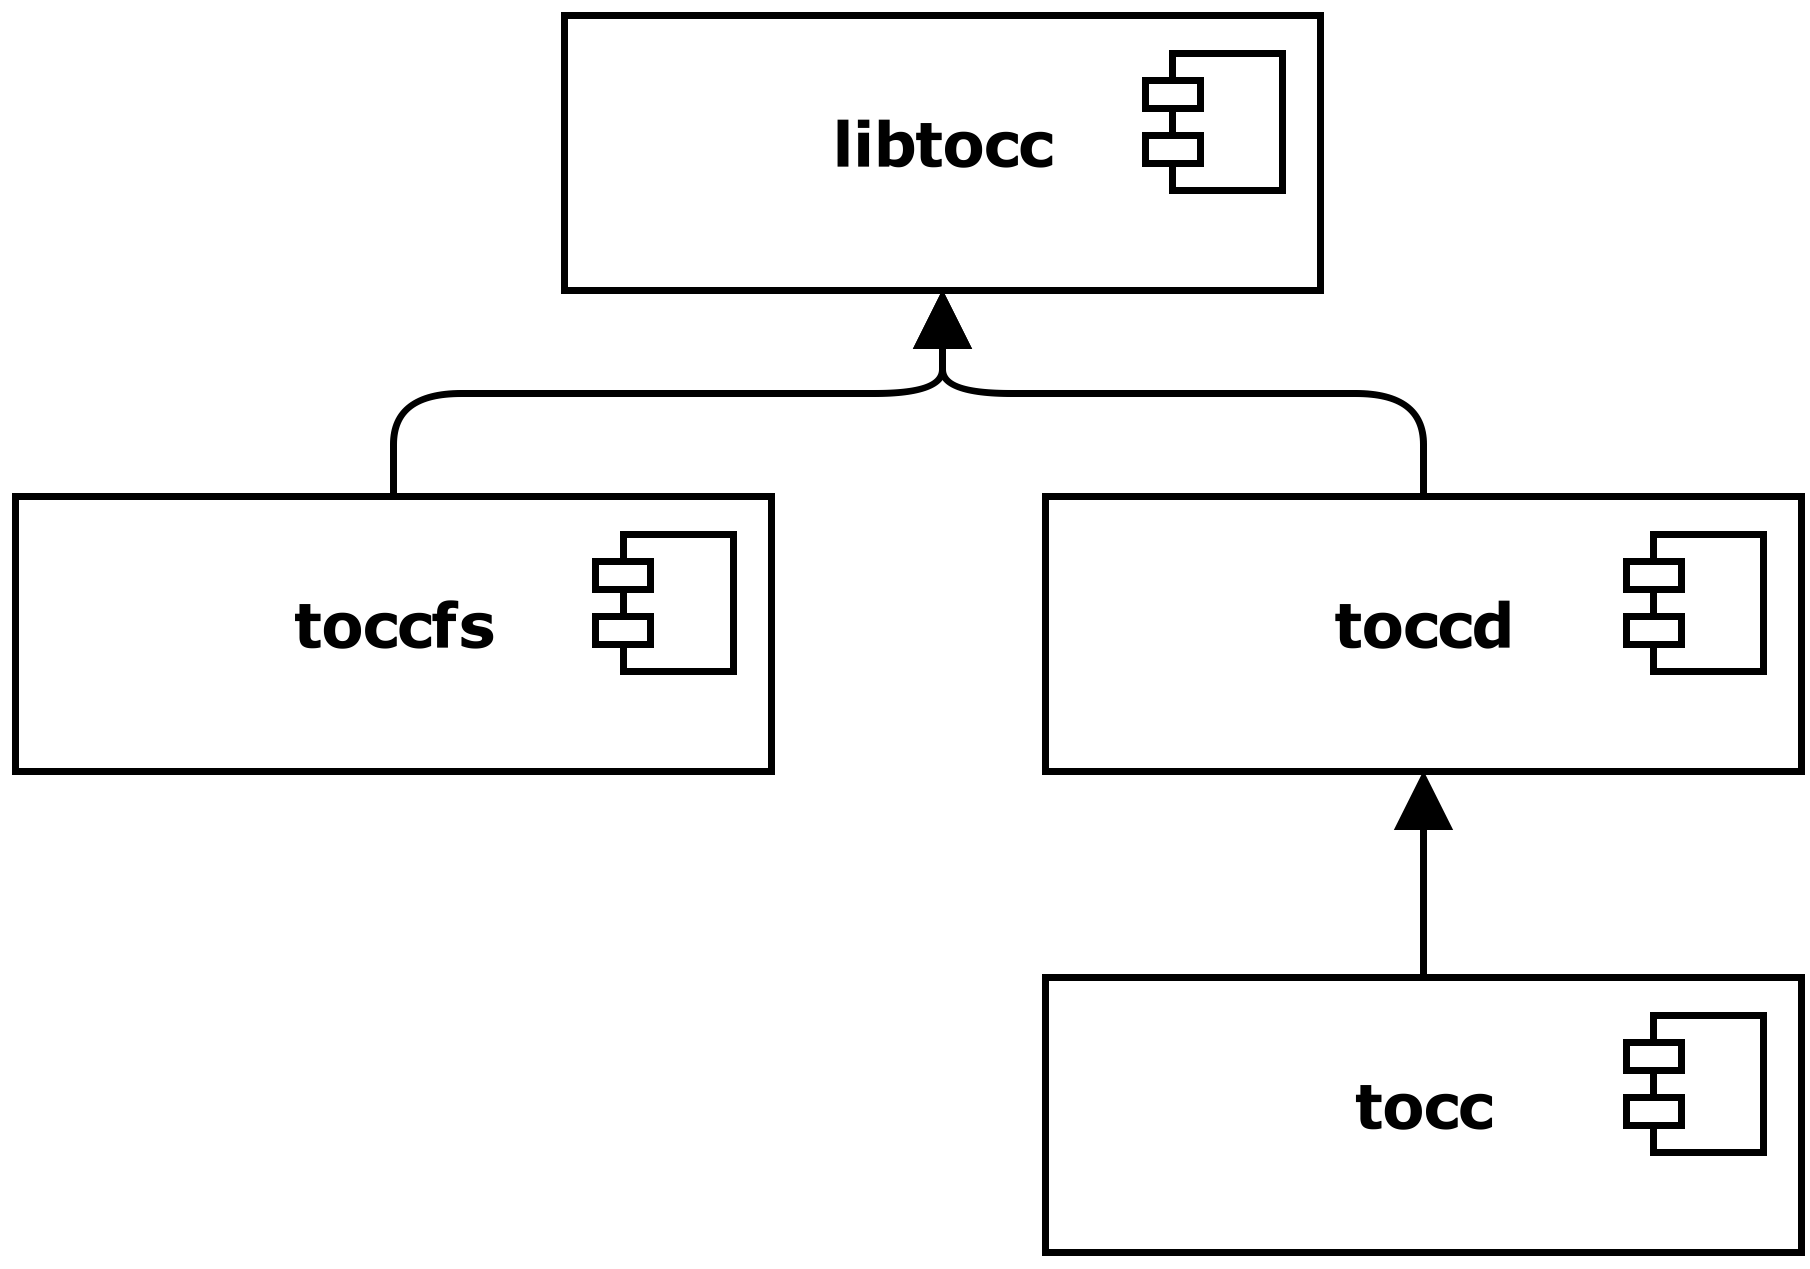
\includegraphics[width=0.9\textwidth]{images/main_components.png}
\caption{main components}
\label{fig:components}
\end{figure}

Everything is implemented in \emph{libtocc}. \emph{toccfs} and \emph{tocc} are two interfaces for the library (there can be more, e.g. a graphical interface).

\emph{toccfs} is a file system written using FUSE\footnote{Filesystem in Userspace \url{http://fuse.sourceforge.net}}. User can interact with it as any other file systems. \emph{tocc} is a command line interface. (\emph{toccd} is there for better performance. It will be explained later.)


\subsection{toccfs}
\emph{toccfs} mounts as a file system in a mount point, and gets a path to were the real files stored. (something like \texttt{toccfs /path/to/files/ /mount/point}). User can use it as a normal file system, i.e. list files in directories, copy or move files, open them, and like that. Each of these commands will be translated into a query passes to \emph{libtocc}.

For example, user may run \texttt{ls photo/abstract/}, and gets all files that tagged photo and abstract. Or, by coping a file to \texttt{black-and-white}, the file will be tagged black-and-white.

\subsection{tocc}
\emph{toccfs} is very limited. If user wants to execute more complicated queries, like searching with Regular Expression, she can use \emph{tocc} command.

\emph{toccd} is a daemon exists for increasing the performance. Since \emph{libtocc} works with a database, each time \texttt{tocc} command executes, a new process will be started and loads database into the memory. If we set aside the time it takes to load the database, the database can't use improvements like caching its data in memory. To solve this, a daemon is running in the background and \emph{tocc} passes its queries to it.

